\documentclass[professionalfonts,compress,unicode,aspectratio=169]{beamer}
\usetheme{Moscow}

\usepackage[utf8]{inputenc}
\usepackage[T2A]{fontenc}
\usepackage[main=russian,english]{babel}

\usepackage{amsmath,amssymb}

\renewcommand{\thefootnote}{\fnsymbol{footnote}}
\hypersetup{pdfauthor={Ivan Tsybulin}}


\graphicspath{{images//}}

\title[Методы Рунге-Кутты]{Задача Коши. Методы Рунге-Кутты. Жесткие задачи}
\author[Цыбулин И.В.]{Скалько Юрий Иванович\\
\textbf{Цыбулин Иван}}
\date{}

\newcommand{\colorhref}[2]{\href{#1}{\textcolor{miptbase!30!black}{#2}}}

\begin{document}

\begin{frame}[plain]
\titlepage
\end{frame}

\renewcommand{\L}{\mathcal{L}}
\renewcommand{\vec}[1]{\boldsymbol{\mathbf{#1}}}
\newcommand{\pd}[2]{\frac{\partial #1}{\partial #2}}
\newcommand{\tr}{\mathsf{T}}

\section{Обыкновенные дифференциальные уравнения}
\begin{frame}\frametitle{Задача Коши}
	Дано обыкновенное дифференциальное уравнение 1го порядка и начальное условие
	\begin{align*}
	\frac{d\vec y(t)}{dt} &= \vec G(t, \vec y(t))\\
	\vec y(0) &= \vec y_0
	\end{align*}
	Требуется найти решение $\vec y(t)$ при $t \in [0, T]$
\end{frame}

\section{Численные методы интегрирования ОДУ}
\subsection{Общие положения}
\begin{frame}\frametitle{Методы Рунге-Кутты}
	\begin{itemize}
	\item
	Методы Адамса относятся к \emph{многошаговым методам}. Для вычисления решения
	$\vec u_{n+1}$ в момент $t_{n+1}$ используется <<история>>, то есть значения
	решения в моменты времени $t_{n}, t_{n-1}, \dots, t_{n-s+1}$. Говорят, что
	такой метод является $s$-шаговым.
	\item
	Методы Рунге-Кутты относятся к \emph{одношаговым методам}, то есть они позволяют по
	значению решения $\vec u_{n}$ вычислить значение в следующей точке $\vec u_{n+1}$.

	Каждый шаг метода состоит из нескольких \emph{стадий}, на которых вычисляются вспомогательные
	наклоны $\vec k$. Вычисление наклонов в специально подобранных промежуточных точках позволяет
	получить метод с высоким порядком аппроксимации.
	\end{itemize}
\end{frame}

\begin{frame}\frametitle{Общая схема методов Рунге-Кутты}
	Каждый метод Рунге-Кутты характеризуется набором коэффициентов $a_{ij}, b_j, c_i$.
	Один шаг метода проводится по следующей схеме:
	\begin{columns}[T]
	\begin{column}{.5\textwidth}
	\begin{align*}
	\vec k_1 = \vec G(t_n + c_1 \tau&, \vec u_n + \tau\sum_{j=1}^s a_{1j} \vec k_j)\\
	&\vdots\\
	\vec k_s = \vec G(t_n + c_s \tau&, \vec u_n + \tau\sum_{j=1}^s a_{sj} \vec k_j)\\
	\frac{\vec u_{n+1} - \vec u_n}{\tau} &= \sum_{j=1}^s b_j \vec k_j
	\end{align*}
	\end{column}
	\begin{column}{.5\textwidth}
	\begin{figure}%
	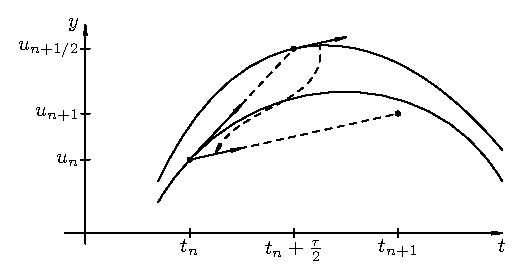
\includegraphics[width=.7\columnwidth]{rk-0.eps}%
	\begin{align*}
	\vec k_1 &= \vec G(t_n, \vec u_n)\\
	\vec k_2 &= \vec G\left(t_n + \frac{\tau}{2}, \vec u_n + \frac{\tau}{2} \vec k_1\right)\\
	&\frac{\vec u_{n+1} - \vec u_n}{\tau} = \vec k_2
	\end{align*}
	\end{figure}
	\end{column}
	\end{columns}
\end{frame}

\begin{frame}\frametitle{Решения, полученные методами Рунге-Кутты}
	Ниже показаны решения задачи о движении тела в поле тяжести, рассчитанные
	различными методами Рунге-Кутты с автоматическим выбором длины шага по
	времени для обеспечения точности $\varepsilon = 10^{-4}$. Точками отмечен
	каждый пятый шаг по времени.

	\begin{figure}
	\centering
	\includegraphics<1>[width=.45\textwidth]{Traj1.png}%
	\includegraphics<2>[width=.45\textwidth]{Traj2.png}%
	\includegraphics<3>[width=.45\textwidth]{Traj4.png}%
	\only<1>{\caption{Метод Эйлера, $3860$ шагов}}%
	\only<2>{\caption{Явный метод центральной точки, $402(\sim 804)$ шагов}}%
	\only<3>{\caption{Метод Рунге-Кутты 4-го порядка, $70(\sim 280)$ шагов}}%
	\end{figure}
\end{frame}

\begin{frame}\frametitle{Таблица Бутчера}
	Коэффициенты $a_{ij}, b_j, c_i$ удобно представлять в виде \emph{таблицы Бутчера}
	\begin{equation*}
	\begin{array}{c|cccccc}
	c_1 & a_{11} & a_{12} & \dots & a_{1s}\\
	c_2 & a_{21} & a_{22} & \dots & a_{2s}\\
	\vdots & & & \ddots & \\
	c_s & a_{s1} & a_{s2} & \dots & a_{ss}\\
	\hline
	& b_1 & b_2 & \dots & b_s
	\end{array}
	\end{equation*}
	\pause
	Например, явному методу средней точки соответствует таблица
	\begin{equation*}
	\begin{array}{c|cccccc}
	0 & 0 & 0\\
	\frac{1}{2} & \frac{1}{2} & 0\\
	\hline
	& 0 & 1
	\end{array}
	\end{equation*}
\end{frame}

\begin{frame}\frametitle{Явные, полуявные и неявные методы Рунге-Кутты}
	В зависимости от коэффициентов $a_{ij}$ вычисления наклонов $\vec k_i$ могут
	происходить по-разному.

	\begin{itemize}
	\item
	Если матрица $a_{ij}$ имеет ненулевые элементы ниже главной диагонали ($a_{ij} = 0, i\geq j$),
	то метод называется \emph{явным}. При этом все наклоны $\vec k_i$ вычисляются через предыдущие без необходимости
	решать уравнения.

	\item
	Если матрица $a_{ij}$ имеет ненулевые элементы и на главной диагонали ($a_{ij} = 0, i > j$),
	то метод называется \emph{полуявным}. При этом все наклоны $\vec k_i$ вычисляются последовательно из уравнений.

	\item
	Иначе, метод называется \emph{неявным}, и необходимо решать систему
уравнений для всех $\vec k_i$ одновременно.
	\end{itemize}
\end{frame}

\subsection{Аппроксимация}
\begin{frame}\frametitle{Разложение наклонов}
	Поскольку метод Рунге-Кутты определяется своими коэффициентами, можно сформулировать условия на коэффициенты метода, при котором
	он имеет определенный порядок аппроксимации. Найдем условия первого и
второго порядков, для этого подставим $\vec u_n = [\vec y]_n$, где $\vec y(t)$ ---
	решение задачи Коши:
	\begin{align*}
	\vec k_i &= \vec G(t_n + c_i \tau, [\vec y]_n + \tau \sum\nolimits_{j=1}^s a_{ij}
\vec k_j) =\\
			&= [\vec G]_n + \tau c_i [\vec G_t]_n + \tau \sum\nolimits_{j=1}^s
a_{ij} [\vec G_y]_n \vec k_j + O(\tau^2) = \\
			&= [\vec G]_n + \tau c_i [\vec G_t]_n + \tau \sum\nolimits_{j=1}^s
a_{ij} [\vec G_y]_n \Big([\vec G]_n + O(\tau)\Big) + O(\tau^2) = \\
			&= [\vec G]_n + \tau c_i [\vec G_t]_n + \tau \sum\nolimits_{j=1}^s
a_{ij} [\vec G_y]_n [\vec G]_n + O(\tau^2)
	\end{align*}
\end{frame}

\begin{frame}\frametitle{Условия первого и второго порядка}
	Выразим производные $\vec y'$ и $\vec y''$ из уравнения:
	$
		[\vec y']_n = [\vec G]_n, \qquad [\vec y''] = [\vec G_t + \vec G_y \vec G]_n
	$
	\begin{align*}
	\vec k_i &= [\vec G]_n + \tau c_i [\vec G_t]_n + \tau \sum_{j=1}^s a_{ij}
[\vec G_y]_n [\vec G]_n + O(\tau^2)\\
	\sum_{j=1}^s b_j k_j &=
	\sum_{j=1}^s b_j [\vec G]_n + \tau \sum_{j=1}^s b_j c_j [\vec G_t]_n + \tau
\sum_{i,j=1}^s b_i a_{ij} [\vec G_y]_n[\vec G]_n \\
	\frac{[\vec y]_{n+1}-[\vec y]_n}{\tau} &= [\vec G]_n + \frac{\tau}{2}[\vec
G_t]_n + \frac{\tau}{2}[\vec G_y]_n [\vec G]_n + O(\tau^2)
	\end{align*}
	\pause
	Условие $1$-го порядка аппроксимации: $\displaystyle \sum_{j=1}^s b_j = 1$.

	Условия $2$-го порядка аппроксимации: $\displaystyle \sum_{j=1}^s b_j c_j = \sum_{i,j=1}^s b_i a_{ij} = \frac{1}{2}$.
\end{frame}

\begin{frame}\frametitle{Автономизация}
	Каждой неавтономной задаче Коши
	\begin{align*}
		&\frac{d\vec y}{dt} = \vec g(t, \vec y)\\
		&\vec y\big|_{t=0} = \vec y_0
	\end{align*}
	можно поставить в соответствие эквивалентную автономную задачу
	\begin{columns}
	\begin{column}{.5\textwidth}
	\begin{align*}
		&\frac{dt}{ds} = 1\\
		&\frac{d\vec y}{ds} = \vec g(t, \vec y)\\
		&\vec t\big|_{s=0} = 0\\
		&\vec y\big|_{s=0} = \vec y_0.
	\end{align*}
	\end{column}
	\begin{column}{.5\textwidth}
	\begin{align*}
		&\frac{d\vec Y}{ds} = \vec G(\vec Y)\\
		&\vec Y\big|_{s=0} = \vec Y_0\\
		&\vec Y = (t, \vec y)^\tr\\
		&\vec G = (1, \vec g)^\tr.
	\end{align*}
	\end{column}
	\end{columns}
\end{frame}

\begin{frame}\frametitle{Правило Кутты}
	Применим метод Рунге-Кутты к автономной системе (заметим, что коэффициенты
$c_i$ для автономной системы не используются)
	\begin{align*}
		&\frac{d\vec Y}{ds} = \vec G(\vec Y)\\
		&\vec Y\big|_{s=0} = \vec Y_0.
	\end{align*}
	Наклоны вычисляются по упрощенным формулам (без явного времени)
	\[
		\vec K_i = \vec G(\vec U_{n} + \tau \sum_{j} a_{ij} \vec K_j) =
\begin{pmatrix}
1\\
\vec g(\vec U_n + \tau \sum_j a_{ij} \vec K_j)
\end{pmatrix}
\equiv
\begin{pmatrix}
1\\
\vec k_j
\end{pmatrix}
	\]
	Заметим, что первая компонента всех $\vec K_i$ всегда равна $1$.
	\[
	\vec U_n + \tau \sum_j a_{ij} \vec K_i = \begin{pmatrix}
t_n + \tau \sum_j a_{ij}\\
\vec u_n + \tau \sum_j a_{ij} \vec k_j
\end{pmatrix}
	\]
\end{frame}

\begin{frame}\frametitle{Правило Кутты}
	В результате применения метода Рунге-Кутты к автономной системе
	\begin{align*}
		&\frac{d\vec Y}{ds} = \vec G(\vec Y)\\
		&\vec Y\big|_{s=0} = \vec Y_0.
	\end{align*}
	получаются формулы, аналогичные методу Рунге-Кутты для системы
	\begin{align*}
		&\frac{d\vec y}{dt} = \vec g(t, \vec y)\\
		&\vec y\big|_{t=0} = \vec y_0.
	\end{align*}
	с тем отличием, что вместо коэффициентов $c_i$ в нем стоят величины $\sum_j
a_{ij}$. Получается, что если имеется метод Рунге-Кутты, имеющий $p$-й порядок
аппроксимации на автономных системах уравнений, универсальный метод Рунге-Кутты
того же порядка получается из него, если положить $c_i = \sum_j a_{ij}$.
Последнее условие называется правилом Кутты.
\end{frame}

\begin{frame}\frametitle{Аппроксимация высших порядков}
	Намного проще выводить условия порядка для автономных систем, так как в этом
случае отсутствуют частные производные по времени.
	\begin{multline*}
	\vec k_i = \vec G([\vec y]_n + \tau \sum_j a_{ij} \vec k_j) = [\vec G]_n
	+ \tau [\vec G_y]_n \sum_j a_{ij} \vec k_j + \frac{\tau^2}{2} [\vec
G_{yy}]_n
	\sum_j a_{ij} \vec k_j \sum_{\ell} a_{i\ell} \vec k_\ell + \\ +
	\frac{\tau^3}{6} [\vec G_{yyy}]_n \sum_j a_{ij} \vec k_j \sum_\ell a_{i\ell} \vec
k_\ell \sum_{m} a_{im} \vec k_m + O(\tau^4).
	\end{multline*}
	Запись $[\vec G_{yyy}]\vec \xi\vec \eta\vec \zeta$ следует понимать как
свертку
	\[
	[\vec G_{yyy}]\vec \xi\vec \eta\vec \zeta = \sum_{j,\ell,m}\pd{{}^3 G_i}{y_j
\partial y_\ell \partial y_m} \xi_j \eta_\ell \zeta_m.
	\]
	В общем случае, за производной порядка $q$ следует $q$ векторов, с которой
она сворачивается. Из-за равенства смешанных производных, порядок векторов не
важен.
\end{frame}

\begin{frame}\frametitle{Аппроксимация высших порядков}
	Из разложения до порядка $O(\tau^4)$
	\[
	\vec k_i = [\vec G]_n + \tau \sum_j a_{ij} [\vec G_y] \vec k_j
	+ \frac{\tau^2}{2} \sum_{j\ell} a_{ij}a_{i\ell}[\vec G_{yy}] \vec k_j \vec k_\ell
	+ \frac{\tau^3}{6} \sum_{j\ell m} a_{ij} a_{i\ell} a_{im} [\vec G_{yyy}] \vec k_j
	\vec k_\ell \vec k_m + O(\tau^4).
	\]
	отбрасыванием степеней можно получить более грубые разложения
	\begin{align}
	\label{eq:third}
	\vec k_i &= [\vec G]_n + \tau \sum_j a_{ij} [\vec G_y] \vec k_j
	+ \frac{\tau^2}{2} \sum_{j\ell} a_{ij}a_{i\ell}[\vec G_{yy}] \vec k_j \vec k_\ell
	+ O(\tau^3)\\
	\label{eq:second}
	\vec k_i &= [\vec G]_n + \tau \sum_j a_{ij} [\vec G_y] \vec k_j +
O(\tau^2)\\
	\label{eq:first}
	\vec k_i &= [\vec G]_n + O(\tau)
	\end{align}
	Подставим \eqref{eq:first} в \eqref{eq:second}:
	\[
	\textstyle
	\vec k_i = [\vec G]_n + \tau \sum_j a_{ij} [\vec G_y]_n ([\vec G]_n + O(\tau))
+ O(\tau^2) =
	[\vec G]_n + \tau \sum_j a_{ij} [\vec G_y \vec G]_n + O(\tau^2)
	\]
\end{frame}

\begin{frame}\frametitle{Аппроксимация высших порядков}
	Постепенно избавляемся от $\vec k_i$ в правой части разложений
	\begin{align}
	\label{eq:4}
	\vec k_i &= [\vec G]_n + O(\tau)\\
	\label{eq:5}
	\vec k_i &= [\vec G]_n + \tau \sum_j a_{ij} [\vec G_y \vec G]_n +
O(\tau^2)\\
	\label{eq:6}
	\vec k_i &= [\vec G]_n + \tau \sum_j a_{ij} [\vec G_y]_n \vec k_j
	+ \frac{\tau^2}{2} \sum_{j\ell} a_{ij}a_{i\ell}[\vec G_{yy}]_n \vec k_j \vec k_\ell
	+ O(\tau^3)
	\end{align}
	В произведении $[\vec G_yy]_n\vec k_j\vec k_\ell$ из \eqref{eq:6} величины $\vec k_j$ u
$\vec k_\ell$ могут быть взяты с погрешностью $O(\tau)$, так как умножаются на
$\tau^2$, а величина $[\vec G_y]_n\vec k_j$ требует значения $\vec k_j$ с точностю
до $O(\tau^2)$ так как умножается всего лишь на первую степень $\tau$.
\end{frame}

\begin{frame}\frametitle{Аппроксимация высших порядков}
	Постепенно избавляемся от $\vec k_i$ в правой части разложений.
	Величины вида $\sum_j a_{ij}$ сразу для краткости заменим на $c_i$:
	\begin{align*}
	\vec k_i &= [\vec G]_n + O(\tau)\\
	\vec k_i &= [\vec G]_n + \tau \sum_j a_{ij} [\vec G_y \vec G]_n +
O(\tau^2) = [\vec G]_n + \tau c_i [\vec G_y \vec G]_n + O(\tau^2)
	\end{align*}
	\begin{multline*}
	\vec k_i = [\vec G]_n + \tau \sum_j a_{ij} [\vec G_y]_n \vec k_j
	+ \frac{\tau^2}{2} \sum_{j\ell} a_{ij}a_{i\ell}[\vec G_{yy}]_n \vec k_j \vec k_\ell
	+ O(\tau^3) = [\vec G]_n + \\ \tau \sum_j a_{ij} [\vec G_y]_n([\vec G]_n + \tau c_i [\vec
G_y\vec G]_n + O(\tau^2)) + \frac{\tau^2}{2} \sum_{j\ell} a_{ij} a_{i\ell} [\vec
G_{yy}]_n ([\vec G]_n + O(\tau)) ([\vec G]_n + O(\tau)) + O(\tau^3) = \\ =
	[\vec G]_n + c_i \tau [\vec G_y\vec G]_n + \tau^2 \sum_j a_{ij} c_j [\vec G_y \vec
G_y \vec G]_n + \frac{\tau^2 c_i^2}{2} [\vec G_{yy} \vec G\vec G]_n + O(\tau^3)
	\end{multline*}
\end{frame}

\begin{frame}\frametitle{Аппроксимация высших порядков}
	На данный момент получены разложения $\vec k_i$ до третьего порядка:
	\begin{align*}
	\vec k_i &= [\vec G]_n + O(\tau)\\
	\vec k_i &= [\vec G]_n + \tau c_i [\vec G_y \vec G]_n + O(\tau^2)\\
	\vec k_i &= [\vec G]_n + \tau c_i [\vec G_y \vec G]_n + \tau^2 \sum_j a_{ij} c_j [\vec G_y \vec
G_y \vec G]_n + \frac{\tau^2 c_i^2}{2} [\vec G_{yy} \vec G\vec G]_n + O(\tau^3)
	\end{align*}
	Проделывая аналогичные подстановки в разложения четвертого порядка, получаем
	\begin{multline*}
	\vec k_i = [\vec G]_n + \tau c_i [\vec G_y\vec G]_n + \tau^2 \sum_j a_{ij} c_j [\vec
G_y \vec G_y \vec G]_n + \frac{\tau^2 c_i^2}{2} [\vec G_{yy} \vec G\vec G]_n +
	\tau^3 \sum_{j\ell} a_{ij} a_{j\ell} c_\ell [\vec G_y \vec G_y \vec G_y \vec
G]_n + \\ +
	\frac{\tau^3}{2} \sum_{j} a_{ij} c_j^2 [\vec G_y \vec G_{yy} \vec G \vec
G]_n +
	\tau^3 c_i \sum_{j} a_{ij} c_j [\vec G_{yy} \vec G_y \vec G \vec G]_n
	+ \frac{\tau^3}{6} c_i^3 [\vec G_{yyy} \vec G \vec G \vec G]_n + O(\tau^4).
	\end{multline*}
	В последнем выражении учтено, что $[\vec G_{yy} (\vec G_{y} \vec G) \vec
G]_n = [\vec G_{yy} \vec G (\vec G_y \vec G)]_n$ из-за симметрии $\vec G_{yy}$.
\end{frame}

\begin{frame}\frametitle{Аппроксимация высших порядков}
	В выражении
	\begin{multline*}
	\vec k_i = [\vec G]_n + \tau c_i [\vec G_y\vec G]_n + \tau^2 \sum_j a_{ij} c_j [\vec
G_y \vec G_y \vec G]_n + \frac{\tau^2 c_i^2}{2} [\vec G_{yy} \vec G\vec G]_n +
	\tau^3 \sum_{j\ell} a_{ij} a_{j\ell} c_\ell [\vec G_y \vec G_y \vec G_y \vec
G]_n + \\ +
	\frac{\tau^3}{2} \sum_{j} a_{ij} c_j^2 [\vec G_y \vec G_{yy} \vec G \vec
G]_n +
	\tau^3 c_i \sum_{j} a_{ij} c_j [\vec G_{yy} \vec G_y \vec G \vec G]_n
	+ \frac{\tau^3}{6} c_i^3 [\vec G_{yyy} \vec G \vec G \vec G]_n + O(\tau^4).
	\end{multline*}
	имеются $8$ разных произведений, сожержащих $\vec G$ и ее производные. Соберем
коэффициенты перед ними в таблицу:

	\begin{center}
	\footnotesize
	\begin{tabular}{c|c|c|c|c|c|c|c|c}
	&$\vec G$ &
	$\tau\vec G_y \vec G$ &
	$\tau^2\vec G_y \vec G_y \vec G$ & $\tau^2 \vec G_{yy} \vec G \vec G$ &
	$\tau^3 \vec G_y \vec G_y \vec G_y \vec G$ &
	$\tau^3 \vec G_y \vec G_{yy} \vec G \vec G$ &
	$\tau^3 \vec G_{yy} \vec G_y \vec G \vec G$ &
	$\tau^3 \vec G_{yyy} \vec G \vec G \vec G$\\\hline
	$\sum_i b_i \vec k_i$ &
	$\sum_i b_i$ &
	$\sum_i b_i c_i$ &
	$\sum_{ij} b_i a_{ij} c_j$ &
	$\sum_i b_i \frac{c_i^2}{2}$ &
	$\sum_{ij\ell} b_i a_{ij} a_{j\ell} c_\ell$ &
	$\sum_{j} b_i a_{ij} \frac{c_j^2}{2}$ &
	$\sum_{ij} b_i c_i a_{ij} c_j$ &
	$\sum_i b_i \frac{c_i^3}{6}$
	\end{tabular}
	\end{center}
\end{frame}

\begin{frame}\frametitle{Аппроксимация высших порядков}
	\begin{center}
	\footnotesize
	\begin{tabular}{c|c|c|c|c|c|c|c|c}
	&$\vec G$ &
	$\tau\vec G_y \vec G$ &
	$\tau^2\vec G_y \vec G_y \vec G$ & $\tau^2 \vec G_{yy} \vec G \vec G$ &
	$\tau^3 \vec G_y \vec G_y \vec G_y \vec G$ &
	$\tau^3 \vec G_y \vec G_{yy} \vec G \vec G$ &
	$\tau^3 \vec G_{yy} \vec G_y \vec G \vec G$ &
	$\tau^3 \vec G_{yyy} \vec G \vec G \vec G$\\\hline
	$\sum_i b_i \vec k_i$ &
	$\sum_i b_i$ &
	$\sum_i b_i c_i$ &
	$\sum_{ij} b_i a_{ij} c_j$ &
	$\sum_i b_i \frac{c_i^2}{2}$ &
	$\sum_{ij\ell} b_i a_{ij} a_{j\ell} c_\ell$ &
	$\sum_{j} b_i a_{ij} \frac{c_j^2}{2}$ &
	$\sum_{ij} b_i c_i a_{ij} c_j$ &
	$\sum_i b_i \frac{c_i^3}{6}$
	\end{tabular}
	\end{center}
	Разложим аналогично $\frac{[\vec y]_{n+1}-[\vec y]_n}{\tau}$:
	\[
	\frac{[\vec y]_{n+1}-[\vec y]_n}{\tau} = [\vec y']_n + \frac{\tau}{2} [\vec
y'']_n + \frac{\tau^2}{6} [\vec y''']_n + \frac{\tau^3}{24} [\vec y^{IV}]_n +
O(\tau^4)
	\]
	и учтем, что
	\begin{align*}
	\vec y'(t) &= \vec G(\vec y(t)) = \vec G\\
	\vec y''(t) &= \frac{d}{dt}\vec G(\vec y(t)) = \vec G_y \vec y'(t) = \vec G_y
\vec G\\
	\vec y'''(t) &= (\vec G_y \vec G)' = \vec G_{yy} \vec G \vec G + \vec G_y
\vec G_y \vec G\\
	\vec y^{IV}(t) &= (\vec G_{yy} \vec G \vec G + \vec G_y\vec G_y \vec G)' = 
	\vec G_{yyy} \vec G \vec G \vec G + 3 \vec G_{yy} \vec G_{y} \vec G \vec G
	+ \vec G_y \vec G_{yy} \vec G \vec G + \vec G_y \vec G_y \vec G_y \vec G
	\end{align*}
\end{frame}

\begin{frame}\frametitle{Аппроксимация высших порядков}
	Допишем в таблицу коэффициенты разожения $\frac{[\vec y]_{n+1}-[\vec
y]_n}{\tau}$
	\begin{center}
	\footnotesize
	\begin{tabular}{p{3em}|c|c|c|c|c|c|c|c}
	&$\vec G$ &
	$\tau\vec G_y \vec G$ &
	$\tau^2\vec G_y \vec G_y \vec G$ & $\tau^2 \vec G_{yy} \vec G \vec G$ &
	$\tau^3 \vec G_y \vec G_y \vec G_y \vec G$ &
	$\tau^3 \vec G_y \vec G_{yy} \vec G \vec G$ &
	$\tau^3 \vec G_{yy} \vec G_y \vec G \vec G$ &
	$\tau^3 \vec G_{yyy} \vec G \vec G \vec G$\\\hline
	$\sum_i b_i \vec k_i$ &
	$\sum_i b_i$ &
	$\sum_i b_i c_i$ &
	$\sum_{ij} b_i a_{ij} c_j$ &
	$\sum_i b_i \frac{c_i^2}{2}$ &
	$\sum_{ij\ell} b_i a_{ij} a_{j\ell} c_\ell$ &
	$\sum_{j} b_i a_{ij} \frac{c_j^2}{2}$ &
	$\sum_{ij} b_i c_i a_{ij} c_j$ &
	$\sum_i b_i \frac{c_i^3}{6}$\\
	$\hspace{-.5em}\frac{[\vec y]_{n+1}-[\vec y]_n}{\tau}$&
	$1$&
	$\frac{1}{2}$&
	$\frac{1}{6}$&
	$\frac{1}{6}$&
	$\frac{1}{24}$&
	$\frac{1}{24}$&
	$\frac{3}{24}$&
	$\frac{1}{24}$
	\end{tabular}
	\end{center}
	Из этой таблицы можно получить условия аппроксимации вплоть до четвертого
порядка. Для этого необходимо приравнять выражения во второй строке со
значениями третьей. Для аппроксимации порядка $p$ нужно оставить только столбцы
с $\tau^q$ где $q < p$.
	\begin{columns}
	\begin{column}{.5\textwidth}
	\begin{align*}
	O(\tau  ) \qquad &\textstyle \sum_i b_i = 1\\
	O(\tau^2) \qquad &\textstyle \sum_i b_i c_i = 1/2\\
	O(\tau^3) \qquad &\textstyle \sum_{ij} b_i a_{ij} c_j = 1/6\\
	O(\tau^3) \qquad &\textstyle \sum_i b_i c_i^2 = 1/3
	\end{align*}
	\end{column}
	\begin{column}{.5\textwidth}
	\begin{align*}
	O(\tau^4) \qquad &\textstyle \sum_{ij\ell} b_i a_{ij} a_{j\ell} c_\ell = 1/24\\
	O(\tau^4) \qquad &\textstyle \sum_{ij} b_i a_{ij} c_j^2 = 1/12\\
	O(\tau^4) \qquad &\textstyle \sum_{ij} b_i c_i a_{ij} c_j = 1/8\\
	O(\tau^4) \qquad &\textstyle \sum_{i} b_i c_i^3 = 1/4
	\end{align*}
	\end{column}
	\end{columns}
\end{frame}


\begin{frame}\frametitle{Барьеры Бутчера}
	Бутчер доказал несколько теорем о связи порядка аппроксимации и количества стадий у методов Рунге-Кутты.
	Явные методы с $s<5$ стадиями могут иметь порядок не выше $s$, но после $s=5$ стадий наступает, так называемый,
	\emph{первый барьер Бутчера}, и порядок аппроксимации не превышает $s-1$. При увеличении $s$ возникают все новые барьеры, понижающие
	порядок аппроксимации.

	Однако, для неявных методов ограничение не такое строгое. Например есть семейство методов (Гаусса), у которых порядок аппроксимации $2s$ при любом числе стадий.
\end{frame}

\subsection{Устойчивость}
\begin{frame}\frametitle{Устойчивость}
	Если правая часть ОДУ $G(t,y)$ липшицева по $y$ с константой $L$
	$$\|\vec G(t,\vec y) - \vec G(t,\vec v)\| \leq L \|\vec y-\vec v\|,$$
	то несложно показать, что константа устойчивости для методов Рунге-Кутты порядка
	$C \sim \exp\{O(L)T\}$. Следовательно, имеет место сходимость решения разностной задачи к решению дифференциальной задачи.

	Но в случаях, когда $LT \gg 1$ константа устойчивости становится огромной.
	Вспомним, что ошибка сходимости связана с ошибкой аппроксимации
	соотношением
	$$\varepsilon_\text{сх} = C	\varepsilon_\text{аппр}(\tau).$$
	Для того, чтобы обеспечить малую ошибку сходимости необходимо выбирать очень
	маленький шаг по времени $\tau$.
\end{frame}

\section{Жесткие задачи Коши}
\subsection{Жесткость}
\begin{frame}\frametitle{Жесткие задачи}
	Жесткие системы ОДУ описывают, как правило, одновременно проходящие очень быстрые и очень медленные процессы. 
	Например, в задачах химической кинетики бывают различия в скоростях реакций до $10^{15}$ раз.
	\pause
	Оказывается, что быстро протекающие процессы, даже быстро закончившись, продолжают влиять на численное решение задачи, 
	вынуждая рассчитывать решение с очень малым шагом по времени, где это, казалось бы, совершенно не требуется (решение довольно гладкое).
\end{frame}

\subsection{Пример жесткой задачи}
\begin{frame}\frametitle{Поле решений жесткой задачи}
	\begin{columns}[T]
	\begin{column}{.5\textwidth}
	\vspace{1in}
	Поле решений уравнения
	\begin{align*}
	\dot x &= -0.5 x + 20 y\\
	\dot y &= -20 y
	\end{align*}
	содержит резкие повороты --- индикатор жесткости задачи.
	\vspace{1in}
	\end{column}
	\begin{column}{.5\textwidth}
	\begin{figure}%
	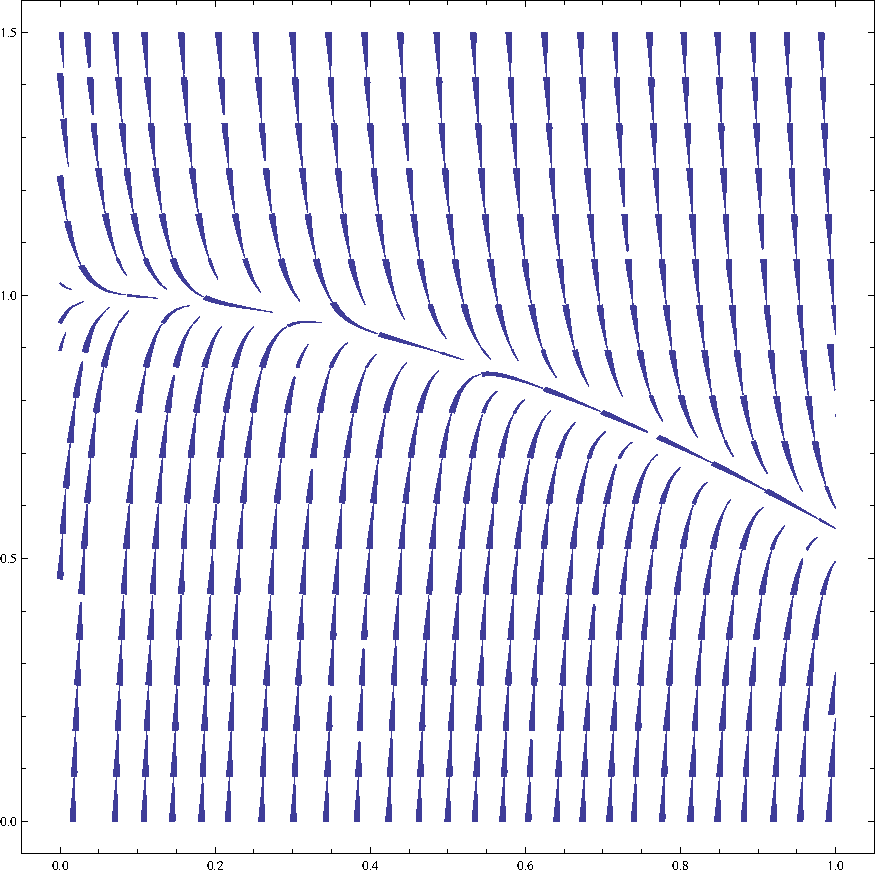
\includegraphics[height=.75\textheight]{stiff.pdf}%
	\end{figure}
	\end{column}
	\end{columns}
\end{frame}

\subsection{Определение жесткой задачи}
\begin{frame}\frametitle{Определение жесткой задачи}
	Можно дать следующее определение:

	Жесткая задача --- это такая задача, у которой собственные числа матрицы Якоби $G_y$
	разбиваются на две части --- мягкую часть спектра $|\lambda_i| < \ell$ и
жесткую часть спектра $\operatorname{Re} \Lambda_i < -L$, причем $\ell \ll L$.
Величина $L/\ell$ называется показателем жесткости.
	\begin{figure}%
	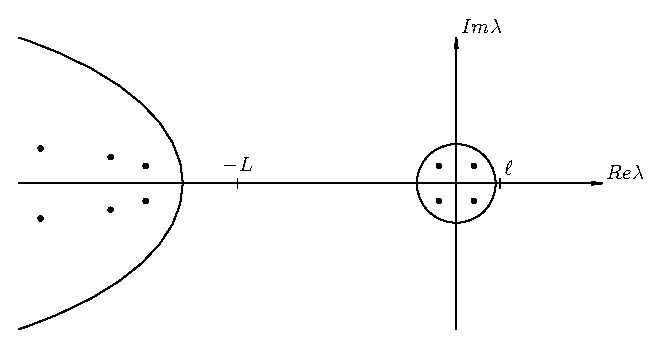
\includegraphics[height=.6\textheight]{sp.eps}%
	\caption{}%
	\label{}%
	\end{figure}
\end{frame}

\subsection{Жесткая устойчивость}
\begin{frame}\frametitle{Модельное уравнение}
	Выяснить, как на жестких задачах себя ведет тот или иной метод, можно на модельном уравнении
	\[
	y' = \lambda y,\quad \operatorname{Re} \lambda < 0
	\]
	Все линейные численные методы для решения этого уравнения будут иметь вид
	\[
	u_{n+1} = r(\lambda \tau) u_n,
	\]
	где $r(z)$ --- функция, зависящая только от метода. Эта функция называется
\emph{функцией устойчивости метода}.
	Если при данном сочетании $\lambda$ и $\tau$ значение функции $r(\lambda \tau)$ по модулю больше единицы, решение будет экспоненциально возрастать, что
	противоречит реальному поведению решения при $\operatorname{Re} \lambda < 0$.
	Область комплексной плоскости $\mathbb{C}$, в которой $|r(z)| < 1$
называется \emph{областью устойчивости метода}.
\end{frame}

\begin{frame}\frametitle{Функция и область устойчивости}
	Если при данном $\tau$ вся жесткая часть спектра попадает в область устойчивости, она гарантированно не будет экспоненциально возрастать, и
	решать систему ОДУ можно только обращая внимание на мягкую часть спектра.

	\begin{columns}[T]
	\begin{column}{.5\textwidth}
	Для явного метода Эйлера
	\[
	\frac{u_{n+1}-u_n}{\tau} = \lambda u_n
	\]
	функция устойчивости
	\begin{align*}
	u_{n+1} &= (1 + \tau \lambda)u_n = (1+z) u_n\\
	r(z) &= 1+z
	\end{align*}
	\end{column}
	\begin{column}{.5\textwidth}
	\begin{figure}%
	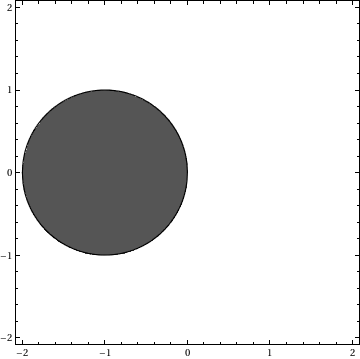
\includegraphics[height=.55\textheight]{euler.png}%
	\end{figure}
	\end{column}
	\end{columns}
\end{frame}

\begin{frame}\frametitle{Область устойчивости}
	\begin{columns}[T]
	\begin{column}{.5\textwidth}
	Для неявного метода Эйлера
	\[
	\frac{u_{n+1}-u_n}{\tau} = \lambda u_{n+1}
	\]
	функция устойчивости
	\begin{align*}
	u_{n+1} &= \frac{u_n}{1 - \tau \lambda} = \frac{u_n}{1 - z}\\
	r(z) &= \frac{1}{1-z}
	\end{align*}
	\end{column}
	\begin{column}{.5\textwidth}
	\begin{figure}%
	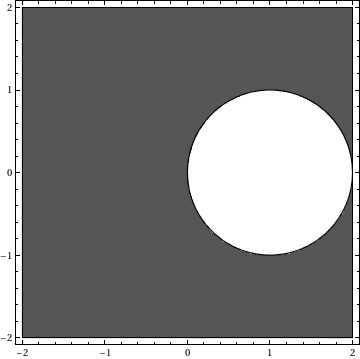
\includegraphics[height=.75\textheight]{euleri.png}%
	\end{figure}
	\end{column}
	\end{columns}
\end{frame}

\begin{frame}\frametitle{Допустимый шаг $\tau$ для жесткой задачи}
	Если шаг по времени $\tau$ таков, что все собственные числа $\Lambda_i$
задачи из жесткой части спектра попадают в область устойчивости данного метода
	\[
		|r(\tau \Lambda_i)| \leq 1,
	\]
	то с таким шагом решать жесткую задачу можно.

	Если это требование нарушить,
жесткие компоненты решения начнут экспоненциально возрастать (хотя обязаны
стремится к нулю!).
	\begin{figure}
	\centering
	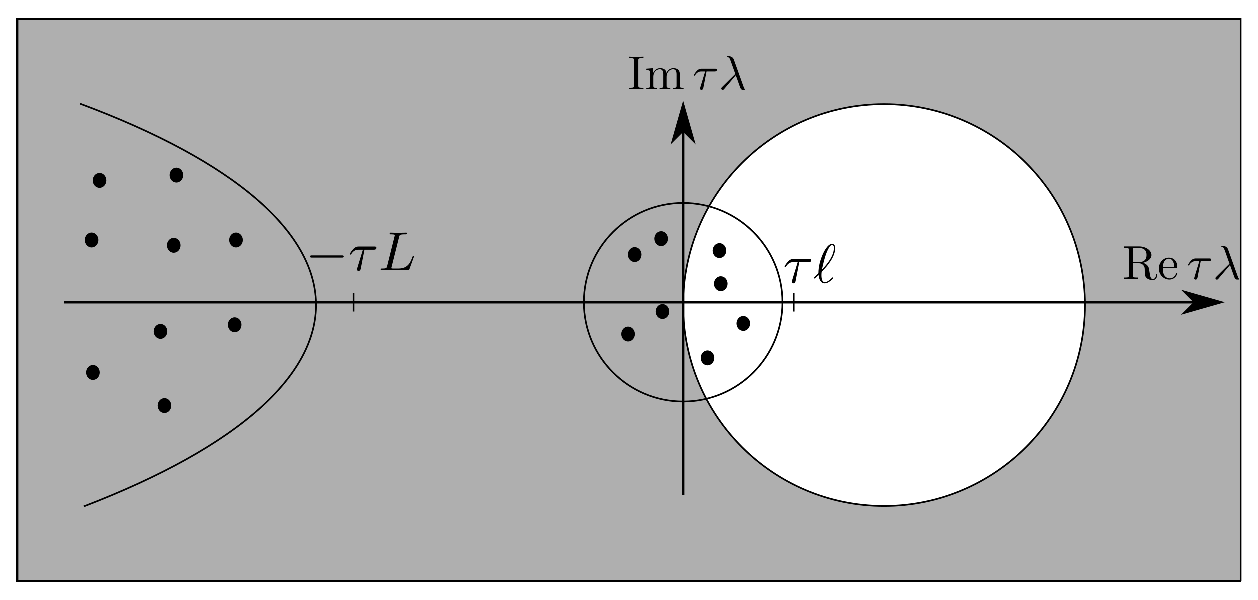
\includegraphics[height=.4\textheight]{stabreg.eps}
	\end{figure}
\end{frame}

\begin{frame}\frametitle[A- и L- устойчивость]{$A$- и $L$-устойчивость}
	По виду области устойчивости методы можно дополнительно классифицировать. Это позволяет выбирать метод,
	наиболее подходящий для конкретного вида жесткой части спектра задачи.

	\begin{itemize}
		\item $A$-устойчивость означает, что во всей полуплоскости $\operatorname{Re} z < 0$ метод устойчив, т.е. $|r(z)| < 1$.
			Такой меотд годится для любых жестких задач.
		\item $A(\alpha)$-устойчивость означает, что в конусе $|\operatorname{Im} z| < -\tg \alpha \operatorname{Re} z$ метод устойчив. $A$-устойчивость 
		эквивалентна $A(90^\circ)$.
			Такой метод годится для задач, у который жесткий спектр прижат к
действительной оси. Чем больше $\alpha$, тем универсальнее метод.
		\item $L$-устойчивость означает, что $\lim_{z \rightarrow -\infty} r(z) = 0$. Это свойство говорит, что при большом шаге $\tau$ жесткая часть спектра 
		стремится к нулю достаточно быстро.
			Эти методы хороши тем, что допускают интегрирование погранслоя с
большим шагом. Не L-устойчивые методы осциллируют при выходе из погранслоя.
	\end{itemize}
\end{frame}

\begin{frame}\frametitle[A- и L- устойчивые методы]{$A$- и $L$-устойчивые методы}
	\begin{figure}
	\centering
	\only<1>{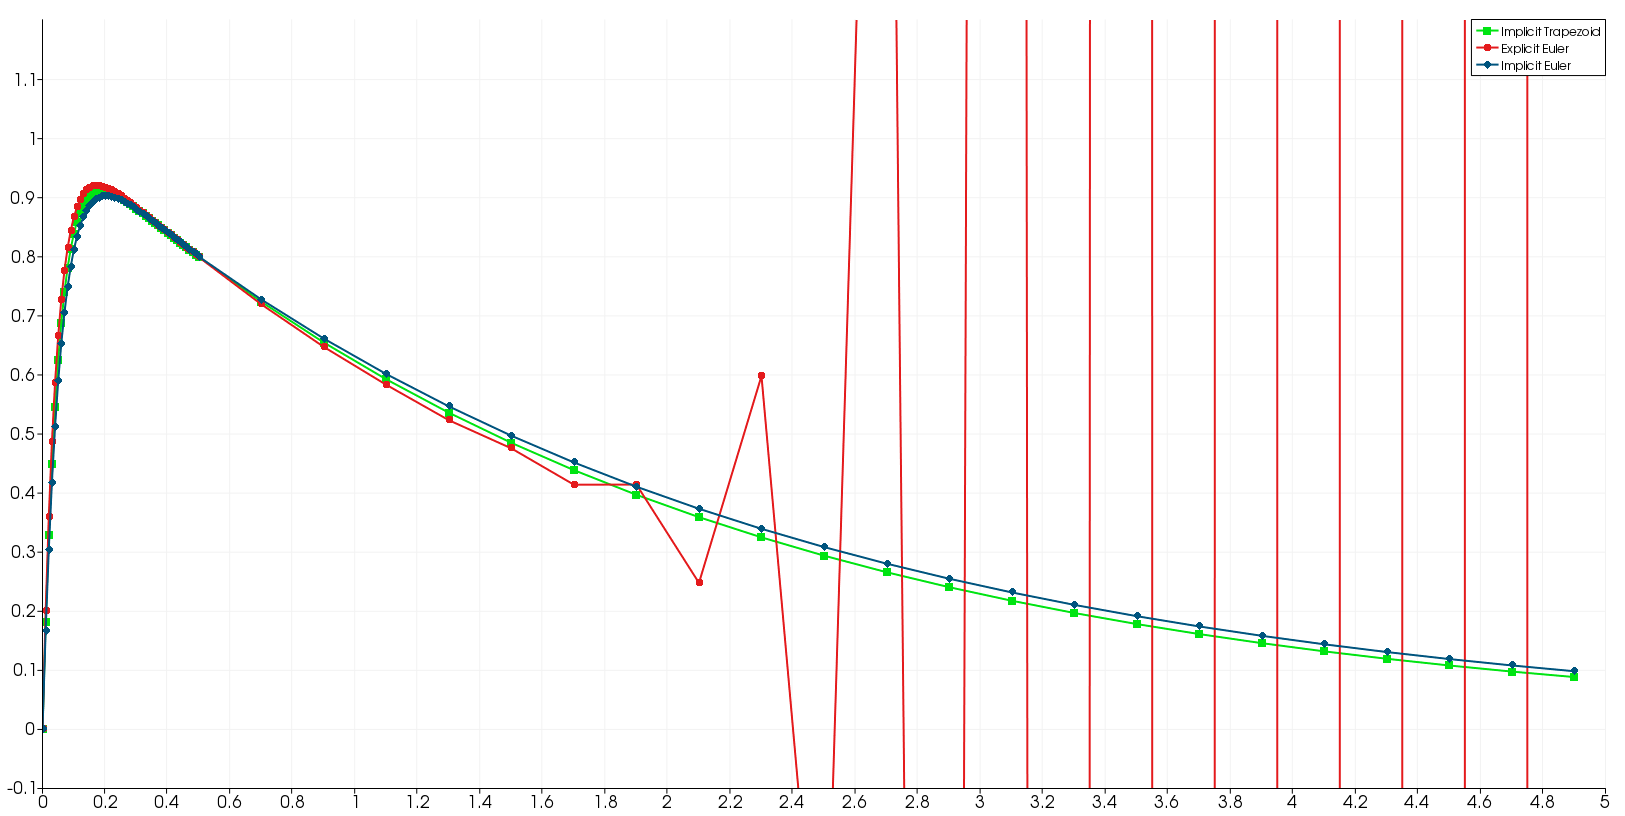
\includegraphics[height=.6\textheight]{fine-coarse.png}}%
	\only<2>{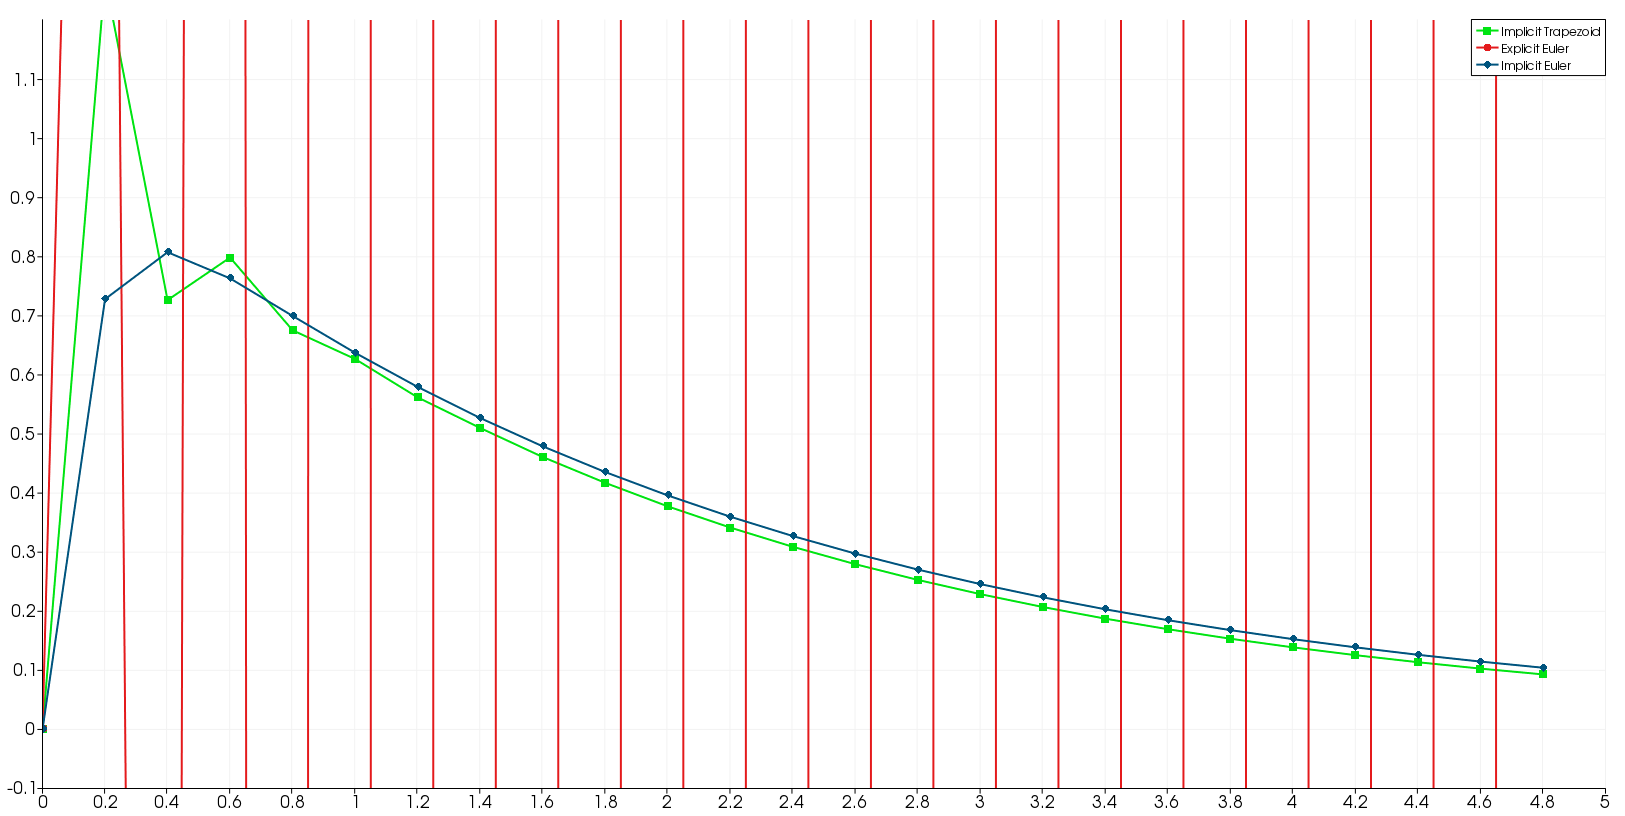
\includegraphics[height=.6\textheight]{coarse.png}}%
	\only<1>{\caption{Решение жесткой задачи разными методами с ограничением шага в
погранслое (красный --- не A-устойчивый явный метод Эйлера, зеленый --- A-, но не
L-устойчивый неявный метод средней точки, синий --- A- и L-устойчивый неявный
метод Эйлера)}}
	\only<2>{\caption{Решение жесткой задачи разными методами с большим шагом
(красный --- не A-устойчивый явный метод Эйлера, зеленый --- A-, но не
L-устойчивый неявный метод средней точки, синий --- A- и L-устойчивый неявный
метод Эйлера)}}
	\end{figure}
\end{frame}

\begin{frame}\frametitle{Функция устойчивости методов Рунге-Кутты}
	Для методов Рунге-Кутты функцию устойчивости можно вычислить по формуле
	\[
	r(z) = \frac{\det(\vec E - z\vec A + z\vec 1\vec b^T)}{\det(\vec E - z\vec A)},
	\]
	где $\vec 1$ --- вектор из единиц.
	\pause
	Для случая явного метода, $r(z)$ является многочленом от $z$ степени $s$ (число стадий).
	Но также, $r(z)$ должен с точностью до $O(z^{p+1})$ совпадать с разложением $e^z$ в ряд по $z$ (аппроксимация порядка $p$).
	Если $s = p$, то $r(z)$ есть просто первые $s+1$ членов ряда Тейлора функции $e^z$.
\end{frame}

\begin{frame}\frametitle{Области устойчивости методов Рунге-Кутты 1--4 порядка}
\begin{figure}%
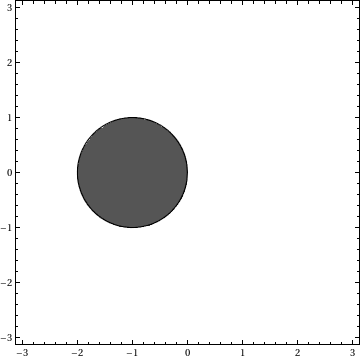
\includegraphics[height=.4\textheight]{rk1.png}%
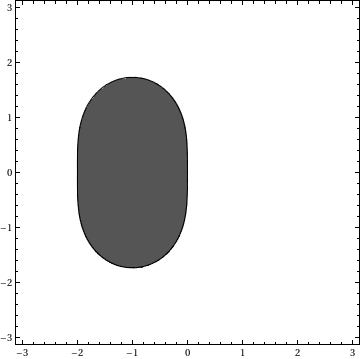
\includegraphics[height=.4\textheight]{rk2.png}%

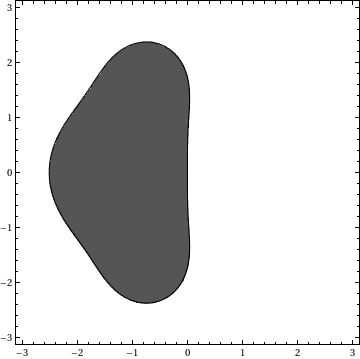
\includegraphics[height=.4\textheight]{rk3.png}%
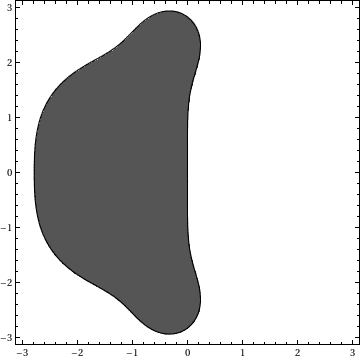
\includegraphics[height=.4\textheight]{rk4.png}%
\end{figure}
\end{frame}

\begin{frame}[plain]
  \begin{center}
  {\Huge Спасибо за внимание!}
  \vspace{8ex}

  Цыбулин Иван

  e-mail: \colorhref{mailto:tsybulin@crec.mipt.ru}{tsybulin@crec.mipt.ru}
  \end{center}
\end{frame}

\end{document}
